\documentclass{standalone}

\usepackage{tikz}
\usepackage{pgfplots}

\usetikzlibrary{calc}

\begin{document}
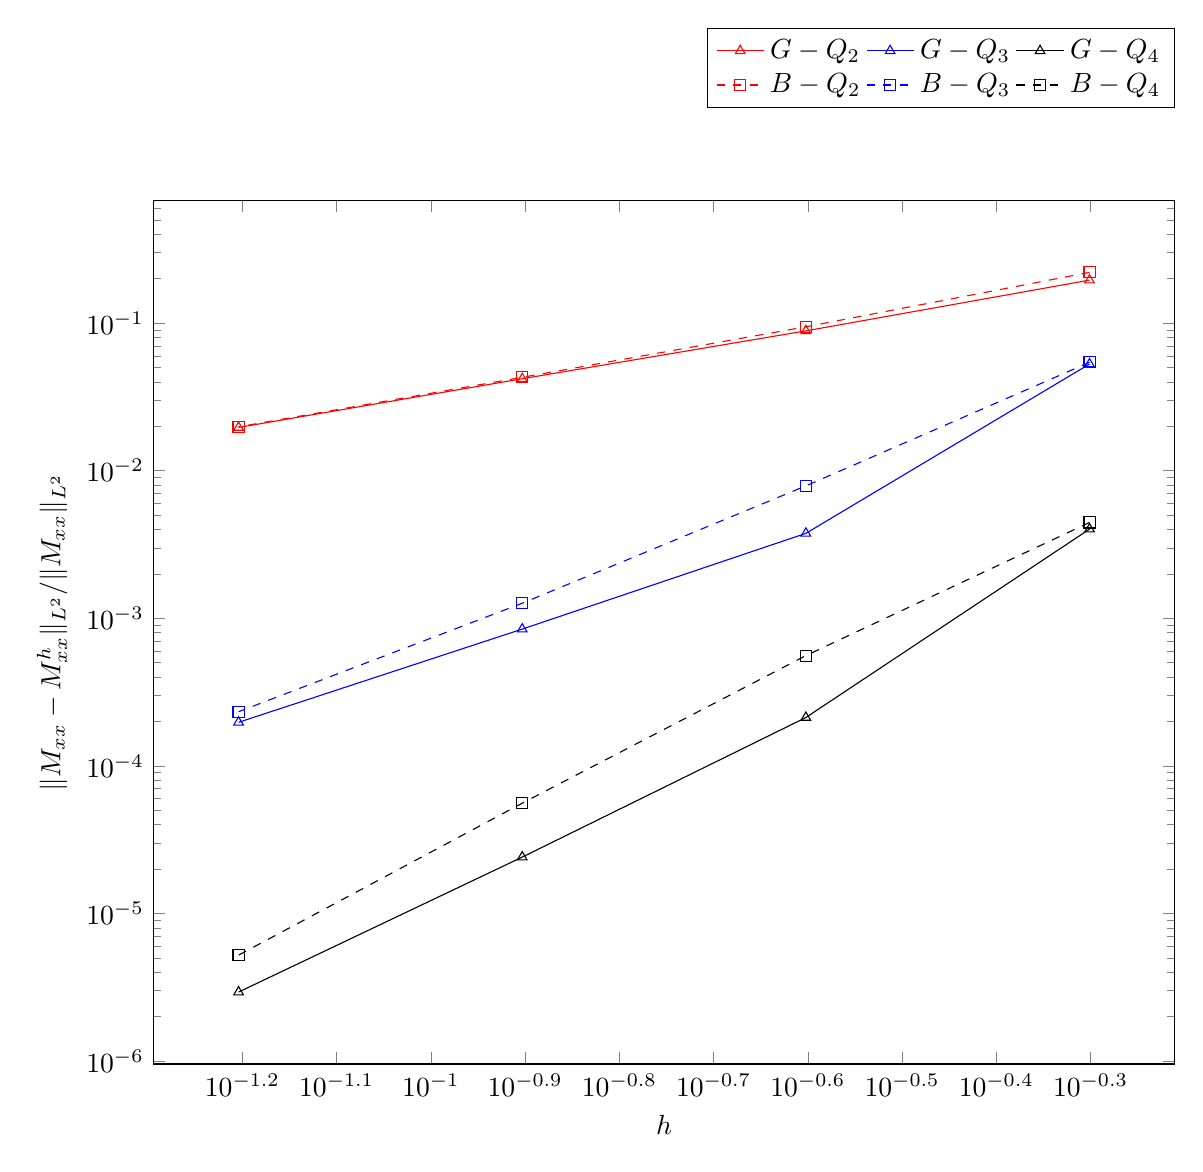
\begin{tikzpicture}
    \begin{loglogaxis}[
        legend columns=3,
    	legend style={at={(1,1.2)}, nodes={scale=1, transform shape}},
        xlabel=$h$,
        ylabel=${\|M_{xx}-M_{xx}^{h}\|_{L^2}}/{\|M_{xx}\|_{L^2}}$ ,
        width=1.2\textwidth
    ]

    \addplot [color=red,mark=triangle] plot coordinates {

        (.5,        0.195378)
        (.25,       0.0885103)
        (.125,      0.0419441)
        (.0625,     0.0196204)
    };

    
    \addplot [color=blue,mark=triangle] plot coordinates {

        (.5,        0.0527854)
        (.25,       0.00376112)
        (.125,      0.000844585)
        (.0625,     0.000197325)
    };

    \addplot [color=black,mark=triangle] plot coordinates {

        (.5,        0.00401614)
        (.25,       0.000212648)
        (.125,      2.40946e-05)
        (.0625,     2.93462e-06)
    };

    \addplot [color=red,mark=square, every mark/.append style={solid}, dashed] plot coordinates {

        (.5,        0.220458)
        (.25,       0.0943194)
        (.125,      0.0428995)
        (.0625,     0.0198136)
    };

    
    \addplot [color=blue,mark=square, every mark/.append style={solid}, dashed] plot coordinates {

        (.5,        0.0542007)
        (.25,       0.00788819)
        (.125,      0.00126382)
        (.0625,     0.000232774)
    };

    \addplot [color=black,mark=square, every mark/.append style={solid}, dashed] plot coordinates {

        (.5,        0.00445847)
        (.25,       0.000558456)
        (.125,      5.58902e-05)
        (.0625,     5.21974e-06)
    };

    \logLogSlopeTriangle{0.25}{0.17}{0.07}{3}{black};
    \logLogSlopeTriangle{0.25}{0.17}{0.38}{2}{blue};
    \logLogSlopeTriangle{0.25}{0.17}{0.72}{1}{red};

    \legend{$G-Q_2$\\$G-Q_3$\\$G-Q_4$\\$B-Q_2$\\$B-Q_3$\\$B-Q_4$\\}
    \end{loglogaxis}
\end{tikzpicture}

\end{document}
